\documentclass{article}
\usepackage{amsmath}
\usepackage{amssymb}
\usepackage{graphicx}
\usepackage{hyperref}
\usepackage[version=4]{mhchem}

\title{Example 9}
\date{}

\begin{document}
\maketitle

(1992 Shanghai Middle School Contest) In square \(A B C D\), shown here, two diagonals meet at point \(E\). The angle bisector of \(\angle C A B\) meets \(B D\) at \(G\), and \(B C\) at \(F\). Find \(F C\) if \(G E=24\).

Solution: 48.
Method 1:\\
\centering
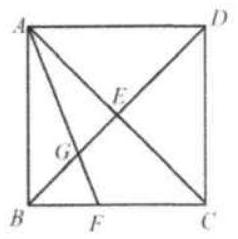
\includegraphics[width=\textwidth]{images/109(2).jpg}

Draw \(F H / / B D\) to meet \(A C\) at \(H . \angle H F C=\angle D B C=\angle H C F=45^{\circ}\). \(H C=F H\).\\
Thus \(\frac{G E}{F H}=\frac{A E}{A H}\)\\
Since \(A F\) is the angle bisector of \(\angle C A B, \angle B A F=\angle H A F, \angle B F A\) \(+\angle B A F=\angle H F A+\angle H A F=90^{\circ} \quad \Rightarrow \quad \angle B F A=\angle H F A\).\\
\centering
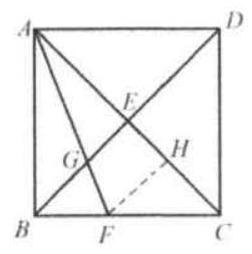
\includegraphics[width=\textwidth]{images/109.jpg}

We know that \(A F=A F\).\\
So \(\triangle A B F \cong \triangle A H F, A H=A B\).\\
Let \(B F=x\). Then \(H C=F H=x, F C=\sqrt{2} x\).\\
\(D C=(1+\sqrt{2}) x\),\\
\(A C=(2+\sqrt{2}) x, A E=\frac{2+\sqrt{2}}{2} x\).\\
(1) becomes: \(\frac{24}{x}=\frac{\frac{2+\sqrt{2}}{2} x}{A C-H C} \quad \Rightarrow \quad \frac{24}{x}=\frac{\frac{2+\sqrt{2}}{2} x}{(2+\sqrt{2}) x-x}\).

Solving we get \(x=24 \sqrt{2}\).\\
\(F C=\sqrt{2} x=48\).\\
Method 2:\\
Draw \(C K / / G E\) to meet the extension of \(A F\) at \(K\).\\
Since \(A E=E C, C K / / G E, C K=2 G F=48\).\\
\(\angle K A C=22.5^{\circ}\).\\
\(\angle A C K=90^{\circ}\). So \(\angle K=67.5^{\circ}\).\\
\(\angle F C K=45^{\circ}\). So \(\angle C F K=67.5^{\circ}\).\\
\centering
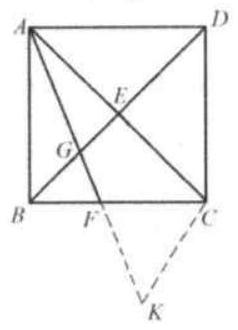
\includegraphics[width=\textwidth]{images/109(1).jpg}

Thus \(F C=C K=48\).


Method 3:\\
Draw \(E H / / F C\) to meet \(A F\) at \(H\).\\
Since \(A E=E C, E H / / F C, F C=2 E H\).\\
Since \(\angle B A F=22.5^{\circ}, \angle A F B=90^{\circ}-22.5^{\circ}=67.5^{\circ}\).\\
Since \(E H / / F C / / B F, \angle E H G=\angle B F G=67.5^{\circ}\)\\
\centering
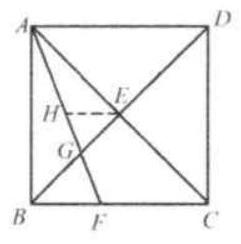
\includegraphics[width=\textwidth]{images/110.jpg}\\
\(\angle E G F\) is the exterior angle of triangle \(A B G\). So \(\angle E G F=22.5^{\circ}+45^{\circ}=67.5^{\circ}=\) \(\angle E H G\).\\
Triangle EHG is an isosceles triangle with \(E H=E G=24\).\\
So \(F C=2 E H=48\).\\

\end{document}
